% (c) Christoph Lange 2007
\documentclass{llncs}

% Draft?
\newif\ifdraft
\drafttrue
%\draftfalse

% \usepackage[english]{babel}
\usepackage[T1]{fontenc}
\usepackage[utf8]{inputenc}
%\usepackage{lmodern}
\usepackage{textcomp}

\ifdraft
\usepackage[show]{ed}
%\usepackage{pdfsync}
\else
\usepackage[hide]{ed}
%\usepackage{microtype}
\fi


% \usepackage{a4wide}
\usepackage{amsmath}
\usepackage{amsfonts}
\usepackage{amstext}
% \usepackage{array}
% \usepackage{graphicx}
% \usepackage{ifthen}
\usepackage{listings}
% \usepackage{lstpatch}
% \usepackage{lstomdoc}
% \usepackage{makeidx}
% \usepackage{scrpage2}
% \usepackage[binary,squaren]{SIunits}
% \usepackage{supertabular}
% \usepackage{tabularx}
% \usepackage{thm2e}
% \usepackage[normalem]{ulem}
\usepackage{wrapfig}
% \usepackage[svgnames]{xcolor}

\usepackage{tikz}

% % Symbol fonts
% \let\RealRightarrow=\Rightarrow
% \usepackage{marvosym}
% \renewcommand{\Rightarrow}{\RealRightarrow}
% \usepackage{wasysym}

% KWARC packages
\usepackage{acronyms,myindex,semantic-markup}
% \let\Realstex=\stex
% \usepackage{paths}
% \renewcommand{\stex}{\Realstex}

% ... and adjustments
\def\omdocni{{\sc OMDoc}} % non-indexed OMDoc
\def\swimni{{\sc SWiM}} % non-indexed SWiM

\hyphenation{name-space}
\hyphenation{Me-dia-Wi-ki}

% Local abbreviations
% \def\abSMW{\product{Semantic MediaWiki}}

% TikZ setup
\usetikzlibrary{arrows}
\tikzstyle{default}=[font=\sffamily,>=triangle 60]
\tikzstyle concept=[font=\sffamily\bfseries,draw,minimum height=3.5ex,rounded corners]

% % Page styles
% \pagestyle{scrheadings}
% \clearscrheadfoot
% \ohead{\headmark}
% \ofoot[\pagemark]{\pagemark}
% \setheadsepline{0.3pt}[\color{gray}]
% \setkomafont{pagehead}{\normalfont\small\sffamily\slshape}
% \setkomafont{pagenumber}{\normalfont\small\sffamily\slshape}
%
% % Listing styles
\lstset{float=htb,columns=flexible,frame=lines,basicstyle=\footnotesize\ttfamily,
        showstringspaces=false,basewidth=.5em}
%
% % Array setup
% \newcolumntype{v}[1]{>{\raggedright\arraybackslash\hspace{0pt}}p{#1}}

\def\thetitle{Flyspeck in a Semantic Wiki -- Collaborating on a Large Scale
Formalization of the Kepler Conjecture}

% load this last
% \definecolor{NavyBlue}{cmyk}{0.94,0.54,0,0.3}
% \usepackage[pdftex,pdfstartview=FitV,plainpages=false,pdfpagelabels,colorlinks=true,linkcolor=NavyBlue,citecolor=NavyBlue,urlcolor=NavyBlue,hypertexnames=true]{hyperref}
% \hypersetup{
%     pdfauthor = {Christoph Lange},
%     pdftitle = {\thetitle},
%     pdfkeywords = {Semantic Wiki OMDoc Ontology Services Science Mathematical
% Knowledge Management Mathematics}
% }
\usepackage{url}

% \hypersetup{bookmarksdepth=4}

\title{\thetitle}
\author{Christoph Lange\inst{1} \and Sean McLaughlin\inst{2} \and Florian Rabe\inst{3}}
\institute{Computer Science, Jacobs University Bremen, \email{\{ch.lange,f.rabe\}@jacobs-university.de} \and
School of Computer Science, Carnegie Mellon University, Pittsburgh, \email{seanmcl@gmail.com}}

\begin{document}

\maketitle

\begin{abstract}
  Semantic wikis have been successfully applied to many problems in knowledge management
  and collaborative authoring.  They are particularly appropriate for scientific and
  mathematical collaboration.  In previous work we described the \textit{OMDoc} semantic
  markup language, and an ontology for mathematical knowledge, and a semantic wiki based
  on both.  We are now evaluating these technologies in concrete application scenarios.

  In this paper we evaluate the applicability of our infrastructure to mathematical
  knowledge management by focusing on \textit{the Flyspeck project}\ednote{@Sean, there
    was a leftover cite{Flyspeck:definition}, which I'd like to move somewhere
    else. --CL}, a formalization of Thomas Hales' proof of the Kepler Conjecture.  The
  Flyspeck project is an ideal target for the semantic wiki framework: It is a relatively
  large project built upon a large number of smaller subprojects that must be organized
  and easily accessible by a diverse audience.

  After describing the Flyspeck project and its requirements in detail, we evaluate the
  applicability of a prototype based on Semantic MediaWiki and of our mathematics-specific
  semantic wiki SWiM to Flyspeck.  Finally, we establish a roadmap on how to improve SWiM
  to better meet the needs of the Flyspeck collaborators.
\end{abstract}

%---------------------------------  Intro: Wiki for Science  -------------------

\section{A Semantic Wiki for Science}
\label{sec:science}

\begin{wrapfigure}{r}{4.2cm}
  \centering
  \vspace{-.9cm}
  \begin{tikzpicture}
    \node (s) at (0,0) {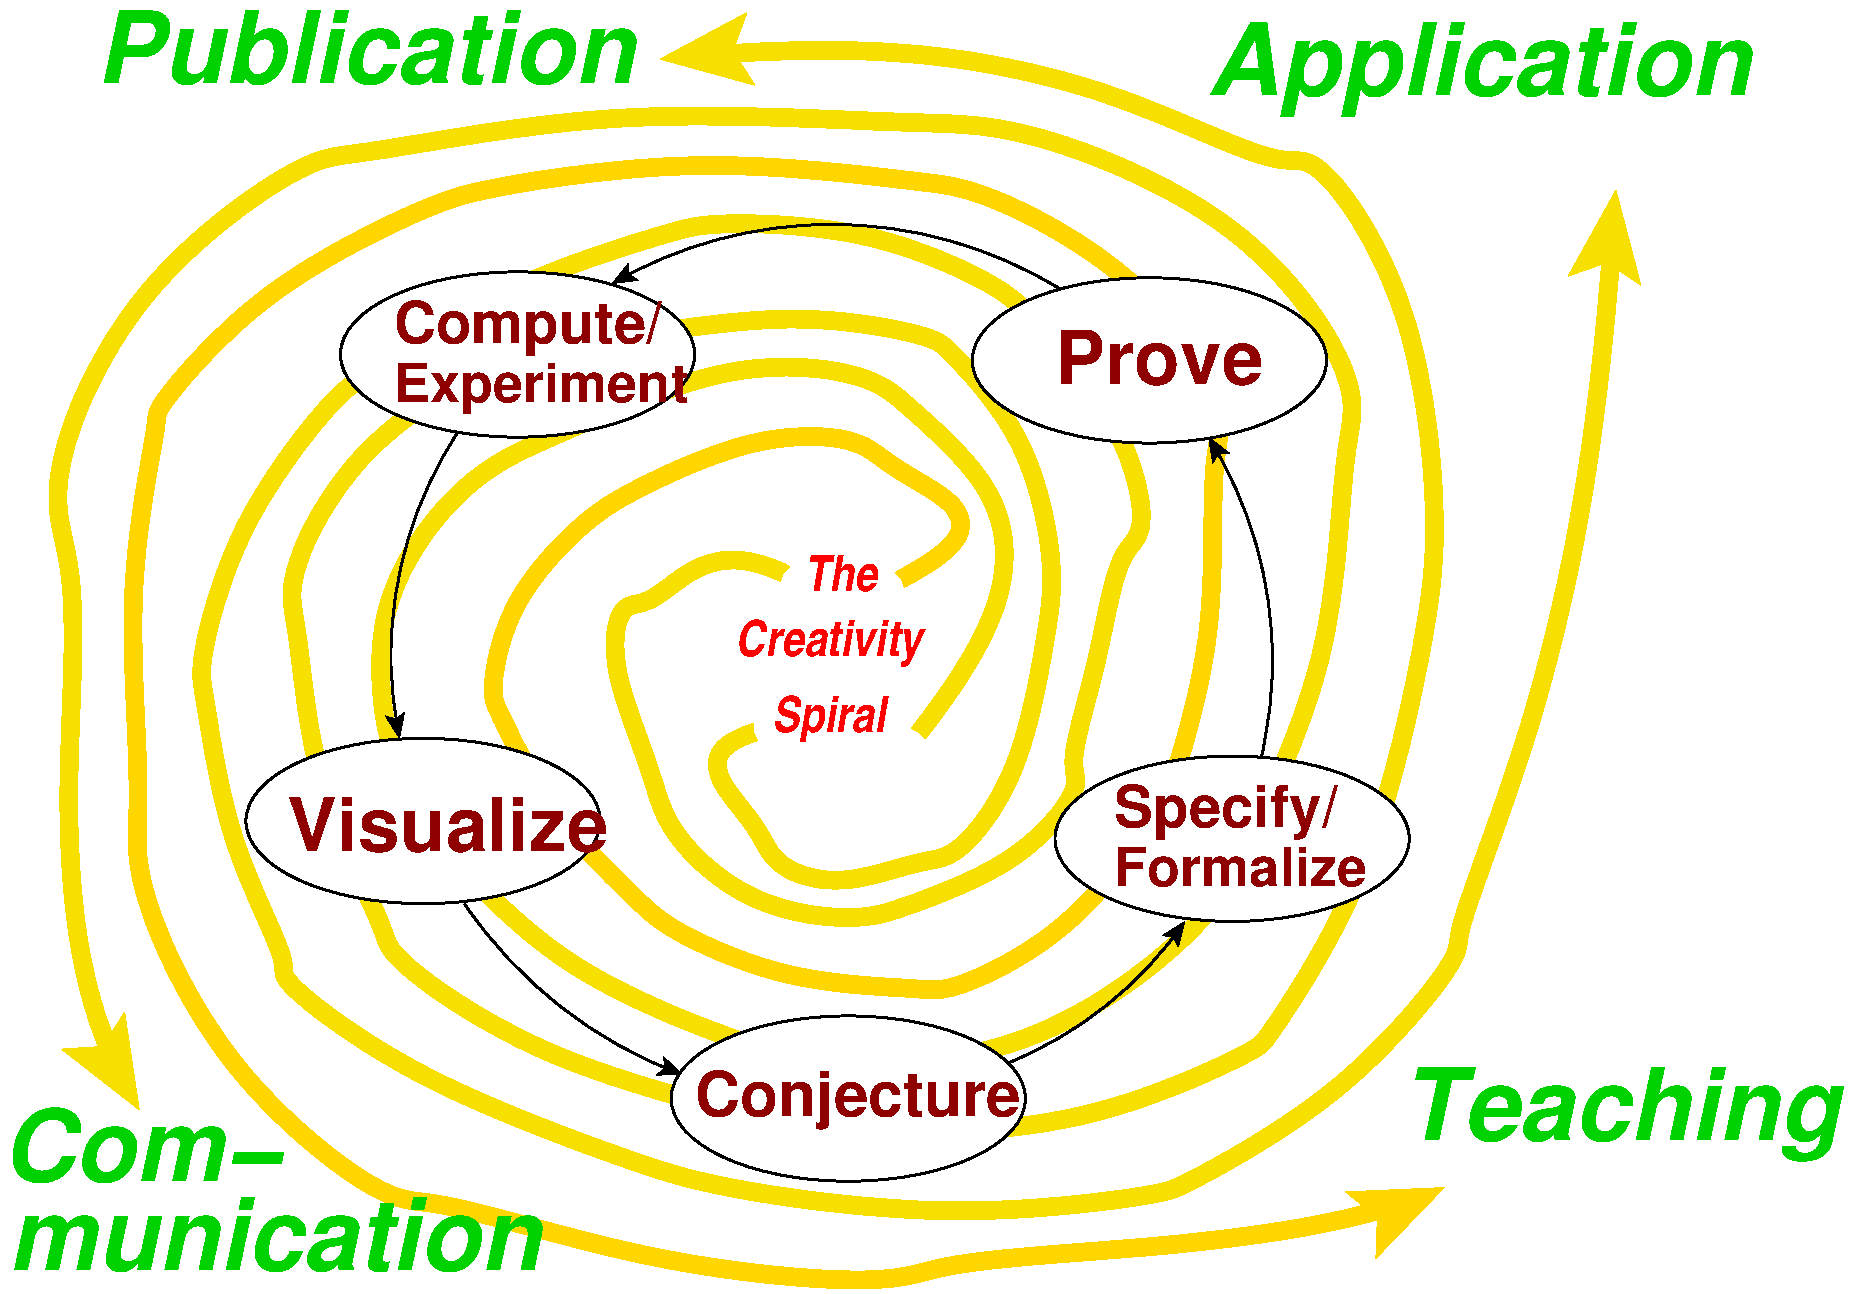
\includegraphics[width=4cm]{images/creativity-spiral}};
    \node at (s.south) {\scriptsize (B.\ Buchberger, 1995)};
  \end{tikzpicture}
  \vspace{-1.2cm}
\end{wrapfigure}
Documents are the most important medium in science, if we assume a broad definition of
``document'', including any materialized item of (scientific) knowledge.  Scientific
communication mainly consists of exchanging documents---from informal drafts circulating
inside a working group to published, well-structured books.  A great deal of scientific
work consists of collaboratively authoring these documents---taking down first hypotheses,
commenting on results of experiments or project steps, as well as structuring, annotating,
and re-organizing existing items of knowledge.  Tools that
\emph{understand} the knowledge contained in scientific documents are desirable for
editing such documents.  One approach towards this is writing scientific documents in a
semantic markup language with an editor that knows the structures available in this
language.

Besides generic approaches like SALT\cite{Groza:SALT07}, the most
extensive work in semantic markup has been in the domain of
mathematics.  This is natural.  Mathematics has a ``long tradition in
the pursuit of conceptual clarity and representational
rigor''\cite{Kohlhase:omdoc1.2}.  Languages like
MathML\cite{CarlisleEd:MathML07}, OpenMath\cite{BusCapCar:2oms04}, and
OMDoc\cite{Kohlhase:omdoc1.2} were developed to present the clearly defined
and hierarchical structures of mathematics in a way that preserves
the intricate relationships.  In this tradition, 
OMDoc is a language that employs Content MathML
or OpenMath for structurally representing mathematical \emph{objects} (symbols,
numbers, equations, etc.).  OMDoc adds two additional layers.  Objects or informal text can
be annotated as mathematical \emph{statements} (symbol declarations, definitions, axioms,
theorems, proofs, examples, etc.), and collections of interrelated statements can be grouped
into \emph{theories}.

With SWiM, a semantic wiki for mathematical knowledge management (see
section~\ref{sec:swim}), we have investigated collaborative editing of OMDoc documents.
It has turned out that a wiki is a suitable tool for supporting the workflow of
incremental formalization inherent to scientific writing.  But wikis have not only shown
to be appropriate for \emph{writing}, but also for project management, e.\,g.\ in
corporate settings\cite{leuf01:wikiway}.  We are therefore interested in applying our
technologies to scientific knowledge engineering projects.  

%% \ednote{I don't think we want this footnote.  It uses space, and if the users
%%   are curious about the difference, which doesn't seem relevant to our papre, they
%%   can look it up.}
%% \footnote{MathML comes in two flavors: Presentation MathML
%%   expresses the way a formula is rendered, whereas Content MathML models its logical
%%   structure.  Formal mathematical software like a Computer Algebra System would export
%%   formulae in Content MathML, but for publishing, they would be converted to Presentation
%%   MathML.} 

%%% Local Variables: 
%%% mode: latex
%%% TeX-master: "flyspeck-wiki-eswc08"
%%% End: 



%---------------------------------  Flyspeck  ----------------------------------

\begin{wrapfigure}{r}{4.2cm}
  \centering
  \vspace{-.95cm}
  \begin{tikzpicture}
    \node (s) at (0,0) {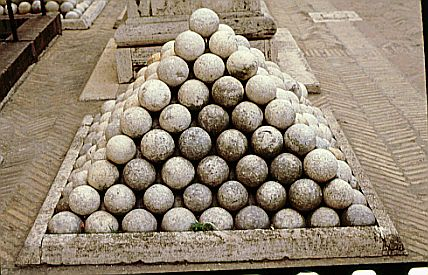
\includegraphics[width=4cm]{images/cannonballs.jpg}};
    \node at (s.south) {\raisebox{-2ex}{\scriptsize (http://tinyurl.com/3bxx2t)}};
  \end{tikzpicture}
  \vspace{-1.0cm}
  \caption{The face centered cubic packing}
  \vspace{-1.0cm}
\end{wrapfigure}
%% alternative images are
%% http://cosmicadventure.com/gallery/albums/album48/Cannonballs_2.jpg
%% http://mathworld.wolfram.com/images/eps-gif/CircleSpherePacking_800.gif
%% http://en.wikipedia.org/wiki/Image:Close-packed_spheres.jpg

\begin{background}
The target of our case study is the Flyspeck Project, which seeks to formally
verify Thomas Hales' proof of the Kepler
Conjecture~\cite{Hales:2005:Annals,Hales:2006:DCG}.  This conjecture asserts
that the density of a packing of unit spheres in 3 dimensions is at most
$\pi/(3\sqrt{2})$, the density of the face centered cubic and hexagonal close
packings.  Posed by Kepler in 1611, it formed part of Hilbert's
18\textsuperscript{th} problem, and until its solution was recognized as one of
the most famous unsolved problems of mathematics.  Hales' proof, completed in
1995, was not accepted immediately by the mathematical community.  Besides its
considerable length, the proof relies essentially on computer calculations.  The
300 pages of text and many thousands of lines of computer code made checking the
proof for errors in the referee process unusually difficult, leading to a
publication delay of nearly 10 years.  In 2003, Hales proposed using computers
to rigorously check the entire proof in detail, including the computer code.  He
dubbed this effort \textit{Flyspeck}\footnote{The word ``flyspeck'' means, ``to
  examine closely''.  It was found by Hales using a regular expression search of
  an English dictionary for the expression ``F.*P.*K'', for ``Formal Proof of
  Kepler''}.  The software systems used in such formalizations are called
\textit{theorem provers} or \textit{proof assistants}\footnote{The word
  ``formalize'' is used in many contexts in this field.  In the remainder of
  this paper, we use ``formal'' and ``formalize'' loosely, possibly referring to
  any degree of colloquial or scientific formalization.  We use ``computerized''
  to mean that a theorem, proof or definition has been expressed in a proof
  assistant.  Note that we consider computerized definitions and proofs formal
  ``documents'' as well.}, examples being Isabelle~\cite{Paulson:1994:Isabelle},
Coq~\cite{Bertot:2004:CoqBook}, and Twelf~\cite{Schurmann:1999:Twelf}.  With
adequate human assistance they can verify that a purported proof follows from a
given set of axioms and inference rules.

Modern proof assistants are still far from being able to check proofs at the
level given in most journals and textbooks.  A typical estimate is that it takes
about a week to formalize a single page of mathematical text.  Hales expects
that it will take around 20 man-years to complete Flyspeck.  Hales is compiling
a {\LaTeX} book~\cite{Hales:2008:FlyspeckBook} of lemmas from different areas of
mathematics that are needed in his proof.  Its 450 pages contain a significant
percentage of the mathematical results used in the proof, covering such
disparate topics as plane, solid, and spherical geometry, graph theory and
hypermaps, single and multivariable calculus, and plane and spherical
trigonometry.

The first steps toward a computerized proof have already been taken.  Nipkow and
Bauer~\cite{Nipkow:2005:Tame} proved the correctness of a fundamental algorithm
in Isabelle.  The other two main parts of the computer code, linear programming
and global optimization, are currently being investigated in doctoral
dissertations~\cite{Zumkeller:2006:TaylorModels,Obua:2005:LinearPrograms}.  A
project page documents some of this progress and has a source repository
containing the book of lemmas, as well as the formalized definitions of some
important functions and inequalities~\cite{website:FlyspeckProjectPage}.
Despite this considerable progress on the computer code, the bulk of the
mathematical formalization remains to be done.  This formalization will consist
of two broad phases.  First, a number of elementary mathematical theories
(e.g. spherical geometry) need to be defined and the relevant lemmas proved.
Then the specific aspects of the Kepler proof that relies on the elementary
results need to be formalized.  Given the content of the book mentioned above,
we suspect that Flyspeck, in its final form, will consist of dozens of theories,
with hundreds of definitions and thousands of lemmas.
\end{background}

\begin{motivation}
\claim{Flyspeck is particularly appealing as a use case for a semantic wiki
approach.}  While the ultimate result is to be a highly formal computerized proof,
the current proof involves both highly formal and semi-formal mathematical
knowledge.  It contains descriptive and motivating yet informal text that should
be preserved for human understanding.  This quasi-formal information would be
difficult to present in a strictly formal setting of a proof assistant.
Secondly, the large number of lemmas, many independent or only loosely coupled,
suggests a ``crowdsourcing'' approach will be beneficial. \claim{Both can be supported
by a (semantic) wiki, as we will show in the following.}
\end{motivation}

%%% Local Variables: 
%%% mode: latex
%%% TeX-master: "flyspeck-wiki-eswc08"
%%% End: 


%-----------------------------  Requirements/Workflow  ------------------------------


\section{Supporting Flyspeck in a Semantic Wiki}

Our focus in this work is on making the extent and structure of Flyspeck
comprehensible, communicating where work needs to be done, and allowing
collaborators to improve the structure and finally to contribute computerized
proofs.  \claim{For this the outline of the whole proof from the
book~\cite{Hales:2008:FlyspeckBook} needs to be represented in the wiki, where
the mathematical statements (including definitions, lemmas, and theorems) are
available in a human-readable way (with formulae in \LaTeX\ or presentational
MathML) as well as a computerized presentation suitable for using in a theorem
prover.}  In order to obtain a well-structured network of knowledge items, each
mathematical statement should be presented on one wiki page, which shows its
human-readable representation taken from the book, offers additional space for
annotation, and allows for downloading a formal representation.  Here, we are
not yet considering formal proof checking \emph{inside} the wiki, but rather
using the wiki for communication about the projects and annotation of informal
text.

% \subsection{Motivation}
% \label{sec:req}

% The Flyspeck project has garnered significant enthusiasm in the theorem proving
% community: Hales has given talks about the project at a number of prestigious
% conferences, and aspects of Flyspeck are currently a motivation behind 
% one complete and at least
% two current PhD dissertations.  At present, however, Flyspeck is not ready for
% crowdsourcing.  

\subsection{Scenario}

\begin{scenario}
An example usage scenario is as follows (cf.\ fig.~\ref{fig:pagestructure}). A
user wishes to contribute to Flyspeck.  She looks at our wiki main page, which
shows her what still needs to be done.  Preferring trigonometry, she searches
for open problems in that field.  This returns a list of lemmas related to
analysis from which she can choose one that seems possible given her time
constraints. She reads the text of a paper proof culled from Hales' book and
annotated by other wiki collaborators and downloads the relevant formal
definitions and lemmas.  She uses a proof assistant to begin formalizing the
paper proof.  At some point, she needs clarification on some definition and
additionally has an idea on how to generalize this lemma.  She thus asks for
help, makes comments on the discussion pages of the wiki, and refines the
annotations of the lemma.  She completes her proof, and uploads the proof
assistant file to the wiki.  The wiki uses a theorem prover to check the proof
for correctness and, if it is correct, adds it to the database.

\newcommand{\wikipage}[6]{\node[draw,text width=4cm,font=\tiny\sffamily,#6] (#1) at #2 {
    {\scriptsize\bfseries #3}\\
    #4
    ~\\[1em]
    [Download Twelf representation]\\
    #5
  };}
\newcommand{\dummywikipage}[2]{\wikipage{#1}{#2}{\textcolor{red!20}{Cosine}}{\textcolor{red!20}{$\cos$}}{
      \textcolor{red!20}{Page type: Definition\\
      Topic: Trigonometry}
    }{fill=red!20}}
\begin{figure}
  \centering
  %\vspace{-.5cm}
  \begin{tikzpicture}[set style={{default}+=[scale=1.5,font=\sffamily]},default,xscale=.8]
    \fill[red!20] (-2.0,-1.0) rectangle (8.1,1.0);
    \wikipage{lemma}{(0,0)}{Lemma 1.3}{The cosine is an even function.\\
      The sine is an odd function.\\
      ${\color{blue}\underline{\cos}}(-x)={\color{blue}\underline{\cos}}(x)$\\
      ${\color{blue}\underline{\sin}}(-x)=-{\color{blue}\underline{\sin}}(x)$}{Page type: Lemma\\
      Topic: Trigonometry\\
      Proven: no (3 attempts)}{fill=red!20}
    \dummywikipage{tan}{(6.2,-0.2)}
    \draw[black!75] (lemma) -- (tan);
    \dummywikipage{sin}{(6.1,-0.1)}
    \draw[black!75] (lemma) -- (sin);
    \wikipage{cos}{(6,0)}{Cosine}{$\cos\colon{\color{blue}\underline{\mathbb{R}}}\to{\color{blue}{\underline{\mathbb{R}}}},x\mapsto\ldots$}{
      Page type: Definition\\
      Topic: Trigonometry
    }{fill=red!20}
    \wikipage{todo}{(0,2.2)}{To do}{Unproven lemmas:
      \begin{tabular}{l|l|l|l}
        Topic & Lemma & Score & Discussion \\
        \hline
        Trigonometry & \textcolor{blue}{\underline{1.3}} & 3 & 5 posts \\
        Hypermaps & 4.2 & \ldots & \ldots 
      \end{tabular}
    }{
      Page type: Overview
    }{}
    \node at (2.5,2.7) {\textcolor{blue}{\underline{1. Browse}}};
    \node[fill=red!20] (d) at (3.5,1.8) {2. Download};
    \draw[->,thick,red!50] (lemma.north east) -- (d);
    \draw[->] (lemma) -- node[above] {usesSymbol} (cos);
    \draw[->] (todo) -- node[left] {references} (lemma);
  \end{tikzpicture}
  \caption{Page Structure and Navigation}
  \label{fig:pagestructure}
  \vspace{-1cm}
\end{figure}
\end{scenario}

\subsection{Requirements}
\label{sec:req}

\begin{contribution}
With this scenario in mind, we propose that the wiki should minimally offer: 
\begin{description}
\item[A knowledge base] of the theory, constant, and lemma definitions.
\item[A theory browser] where a user can browse the knowledge by category, or search with keywords.
\item[An editor] to annotate and structure informal texts on their way to
  computerization.
\item[A download area] where one can download existing computerized definitions,
  lemmas, and proofs.
\item[An upload area] where one can upload new proofs.
\item[Discussion pages] to discuss issues involved in the formalizations.
\end{description}

The following set of annotations should support this minimal infrastructure:

\begin{description}
\item[Categorization by topic:] In the beginning, one would mirror the narrative structure
  of the book (e.\,g.\ ``sphere'' being a subsection of ``primitive volumes'', which in turn
  is a section of the chapter ``volume calculations'').  Standardized ways of classifying
  mathematical topics, such as the Mathematical Subject Classification
  (MSC)~\cite{AMS:MSC2000}, could be added later.
\item[Project-organization metadata] such as whether the proof
  of a lemma has already been computerized, or if someone is currently 
  attempting a proof.  This is essential so that two people do not duplicate
  work.
\item[Dependency links:] These can be links from individual symbols in
  mathematical formulae to the place where they are declared, or from any page
  $p$ to other pages containing knowledge that is required for understanding
  $p$: either pages in the same wiki, or external resources like PlanetMath or
  Wikipedia articles.  Authors should be able to add them where they are
  missing.
\item[Discussion posts] should be strongly tied to the topic being
  discussed, and classified into categories like question, answer,
  explanation, etc.
\end{description}

An enticing page for visitors and potential collaborators should give an
impression of the extent and structure of the project (e.\,g.\ its size and its
specialization into diverse fields of mathematics).  For the developer, there
should be tools for browsing and querying the knowledge.  Not only should it be
possible to query knowledge items by their annotations, but important query
results must also be available as dynamically generated lists.  Examples for
queries are:

\begin{enumerate}
\item\label{item:proven-lemma} ``Which lemmas about composite regions need
  to be proved?''
\item ``What lemmas are difficult to prove?''
  \begin{enumerate}
  \item \ldots in the sense that many people have already attempted them, but given up
  \item\label{item:question-count} \ldots in the sense that many people have asked
    questions in the related discussion
  \end{enumerate}
\item ``Are there textual resources I can read in order to understand the Jordan
  Curve Theorem?''
\item ``What other lemmas could help me to prove this one?'' (e.\,g.\ because
  they prove a related statement)
\end{enumerate}

A volunteer who is willing to work out and contribute a computerized proof for a
lemma should be able to download a self-contained computerized representation of
this lemma and everything it depends on.  Different notions of ``dependency''
can be supported, the most straightforward being that a lemma depends on the
declarations and definitions of all symbols it uses and on the transitive
closure of all symbols used by the latter.  Related lemmas could be downloaded
and assumed as axioms, under the assumption that those will be proved later,
perhaps by other collaborators.  Finally, assuming that the Flyspeck
book~\cite{Hales:2008:FlyspeckBook} is written in a linear order, \emph{all}
definitions and lemmas before the current one in the narrative order could be
used.  

\claim{During the formalization of the knowledge, we anticipate that the definitions
will undergo refactoring in order to facilitate the actual development of the
proofs.}  (Historically, this has been the case with many large computerized
proofs, cf.~\cite{Gonthier:2005:FourColor}.)  Refactoring support by the wiki
would thus be advantageous.  In fact, as definitions rely so heavily on each
other, and the lemma statements rely on the definitions, Hales needs to oversee
the computerization of the definitions so that the mathematical constants are
correct\footnote{For example, one can represent a vector as a function from the
  integers to the reals, or as a tuple of reals.  The operations of vector
  spaces will depend on this representation, etc.}.  This could be done by
allowing him and other experienced mathematicians to \emph{rate} the
contributions of the collaborators.
\end{contribution}

%%% Local Variables: 
%%% mode: latex
%%% TeX-master: "flyspeck-wiki-eswc08"
%%% End: 


%-----------------------------  Case Studies  ------------------------------

\section{Case Studies and Evaluation}

So far, the Flyspeck project has four core members who collaborate via
GoogleCode\cite{website:FlyspeckProjectPage}.  While the services offered by
GoogleCode (a Subversion repository, a mailing list, and others) were
found to be sufficient for the core development team, we were not
satisfied with the wiki integrated into the GoogleCode web interface.
Lacking support for mathematical formulae, it would not even allow for
presenting the theorems and lemmas to be formally proven in a
human-readable fashion.  Furthermore, GoogleCode offers very
little \emph{structuring} support, which we believe will be
essential for browsing and querying Flyspeck's 
(eventually) large knowledge collection.  We sought to improve
on GoogleCode with two prototypes.  
In the following sections, we evaluate the prototypes 
for their applicability to Flyspeck with regard to their
support for annotations, browsing, and querying, as specified in
section~\ref{sec:req}.  For the case study, we took a simplified 
view of Flyspeck, using only the {\TeX} sources of the
Flyspeck book and a Twelf formalization of the first chapter (Trigonometry).
The goal was to present the trigonometry chapter in a compelling way
that we believed would scale 2-3 orders of magnitude.  

Both systems are semantic wikis, where one resource (in the RDF sense)---e.\,g.\
one mathematical theorem---is represented by one wiki page and relations between
resources by links between pages.  Both pages and links can be typed with terms
from ontologies\cite{OrDeMoVoHa06:annotation-navigation-semwiki}, which are
either preloaded into the wiki or modelled
ad-hoc\cite{KrSchVr:semwiki-reasoning07}.  This is the prevalent approach of
adding semantics to wikis, although other ways have been
investigated\cite{semwiki06}.  Semantic wikis offer enhanced navigation
capabilities.  For example, they can usually display a summary of all typed
links, grouped by type, for each page.  They support searching for pages by type
or by a page being source or target of a typed link\footnote{Both explicit and
  inferred links (= RDF triples) can be
  considered\cite{KrSchVr:semwiki-reasoning07}}.  Such queries can usually be
executed interactively, or in an automated way as \emph{inline} queries embedded
into the content of a page\cite{KrSchVr:semwiki-reasoning07}.  Both systems we
consider support this basic set of semantic wiki features.

\subsection{Semantic MediaWiki 1.0}
\label{sec:smw-study}

Semantic MediaWiki\cite{KrSchVr:semwiki-reasoning07} is a semantic web extension
to MediaWiki, the system driving \product{Wikipedia}.  Plain MediaWiki supports
mathematical formulae written in {\LaTeX} and allows for categorizing pages.
Semantic MediaWiki interprets category membership as an instance-of relationship
and supports the creation and editing of typed links (called properties).
External ontologies can be referenced from the wiki, but at most sites powered
by Semantic MediaWiki, site-specific ontologies are developed in an ad-hoc
manner\cite{ontoworld:sites-using-smw}.

\paragraph{Prototype} In Semantic MediaWiki, we imported the Twelf master source
of Flyspeck via a customly implemented special page.  The Twelf file was first
enhanced by special comment lines marking the beginning and end of a declaration
with information about topical categorization.  The Twelf upload special page
handler breaks an uploaded file down into declarations and creates two wiki
pages for each Twelf declaration: one page that just contains the Twelf listing,
categorized in the OMDoc document ontology (e.\,g.\ \textit{Lemma}; see
section~\ref{sec:swim}), and one container page that includes the Twelf page via
MediaWiki's template inclusion mechanism, but also allows for including a
{\LaTeX} representation and leaves space for free-form annotations made by the
contributors.  Additionally, MediaWiki offers a discussion page for each page of
mathematical content.  The Twelf pages are overwritten on every import from the
master source, whereas existing container pages remain untouched.  This allows
one to change the computerized version of a Twelf constant in the master source
(e.\,g.\ if it is incorrectly specified) and reimporting it without losing the
semantic markup and comments.

As a first step, we separated symbols and lemmas, which are treated equally in Twelf, by starting lemmas with
``lemma-''. Additionally, the
upload extension recognizes all previously imported symbols in Twelf expressions
and turns them into links of the type \textit{Statement--uses--Symbol}.\ednote{FR: I have no idea what this sentence means.}

\begin{figure}
  \centering
  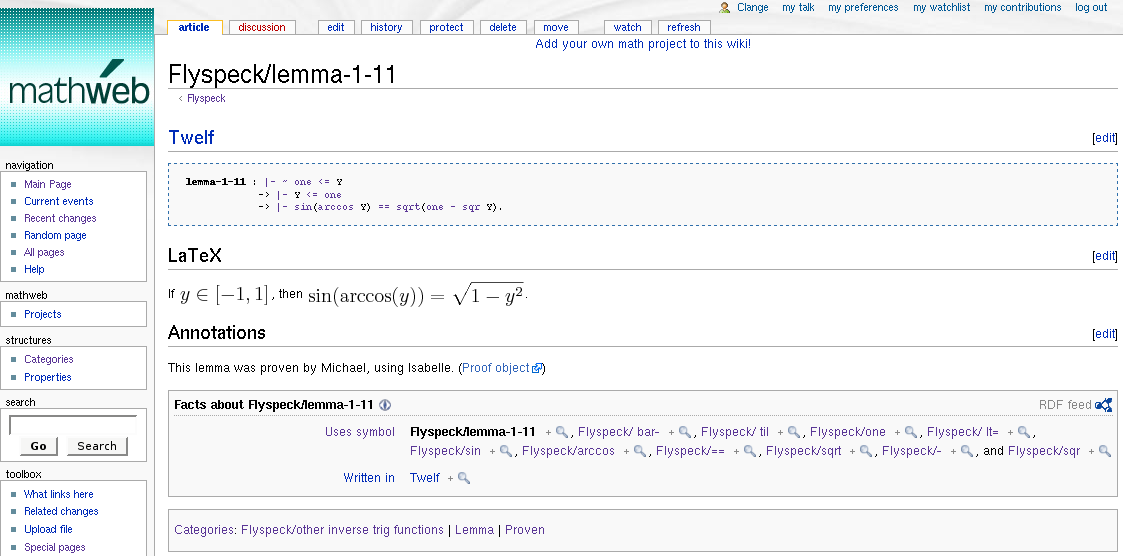
\includegraphics[width=\textwidth]{images/smw-lemma}
  \caption[A Flyspeck lemma in Semantic MediaWiki]{A Flyspeck lemma in Semantic
    MediaWiki\protect\footnotemark}
  \label{fig:smw-lemma}
\end{figure}
\addtocounter{footnote}{-1}
\stepcounter{footnote}\footnotetext{See \url{http://mathweb.org/wiki/Flyspeck}}

The annotations generated that way can be used for browsing, either via the
``fact box'' (the summary of all typed links), or by the special ``browse''
page.  For querying, Semantic MediaWiki offers a simple triple search, as well
as inline queries.  The query language corresponds to the description logic
$\mathcal{EL}^{++}$\cite{KrSchVr:semwiki-reasoning07}, which, for example, does
not support negation.  A query for unproven lemmas about a certain topic could
only be performed if the ``unprovenness'' were explicitly annotated.  The
following queries additionally ask for lemmas available in a Twelf formalization:

\begin{lstlisting}
<ask>[[Category:Unproven]] [[Category:Lemma]]
     [[Category:Trigonometry]] [[written in::Twelf]]</ask>
\end{lstlisting}

Exporting computerized representations of knowledge items is not yet supported
conveniently.  The Twelf listings can be viewed on their own pages, but due to
the auto-generated symbol links in the source code, these are not suitable for
download.  One would either have to implement a special Twelf download page that
cleans these sources again, or one would have to implement the symbol linking as
an extension of the rendering process.

\paragraph{Evaluation} We found the ad-hoc ontology development useful while
prototyping the annotations that might be required for Flyspeck, e.\,g.\
project-related metadata like the information whether a lemma has already been
proven, or categorization by topic.  Semantic MediaWiki did not meet the
requirements in places where ontologies already existed.  For example, in
structures of mathematical documents, it was possible to reference
\emph{vocabulary} from the OMDoc document ontology, but not to apply further
inference rules given there to items of mathematical knowledge.  This is because
Semantic MediaWiki does not support a full \emph{import} of external ontologies.
Most annotations were modelled by categorization, i.\,e.\ instantiation of
classes---certainly not the most formal way of structuring knowledge in view of
many classes just corresponding to narrative sections of the book, but the one
that is supported best by Semantic MediaWiki.

Semantic MediaWiki does not understand the semantics of mathematical formulae,
as the {\LaTeX} formulae cannot be annotated.  The Twelf listings could be
annotated, but at the cost of making them harder to download.

The inline queries were intuitive to write but not as powerful as required.
Complex reasoning tasks like inference of dependencies are not possible in
Semantic MediaWiki; in the restricted domain-specific setting of Flyspeck one
could realize them by hard-coded extension functions.

\subsection{SWiM 0.2}
\label{sec:swim}

SWiM is a semantic wiki targeted at mathematical knowledge management.  Based on
the general-purpose semantic wiki
\product{IkeWiki}\cite{KrSchVr:semwiki-reasoning07}, it adds support for
browsing, editing, rendering, importing and exporting mathematical documents
written in OMDoc.  The semantics of mathematical knowledge is mainly captured in
the OMDoc markup, and more explicitly in a \emph{document ontology}: Whenever a
wiki page containing OMDoc fragments is saved, its type and its (typed)
relations to other items of mathematical knowledge in the wiki are extracted
from the OMDoc XML markup and explicitly represented as RDF triples using terms
of the OMDoc document ontology\cite{OMDocDocOnto:web}.  This ontology models
those aspects of the three layers of mathematical knowledge supported by OMDoc
to the extent supported by the expressivity of OWL-DL\cite{McGvHa:owl04}.
Modeling all modules of the OMDoc specification in this ontology is work in
progress; so far, most mathematical statements as well as key aspects of
theories have been implemented.  Relevant classes for Flyspeck would be
\textit{Lemma}/\textit{Theorem}/\textit{Corollary}/\ldots (all being subclasses
of \textit{Assertion}), \textit{Proof}, \textit{Symbol} (a symbol declaration),
\textit{Definition}, and the properties \textit{Proof--proves--Assertion} and
\textit{Symbol--hasDefinition--Definition}.

\begin{figure}
  \centering
  \begin{tikzpicture}[set style={{default}+=[xscale=.5,yscale=.47,font=\normalsize\sffamily]},default]
    \tikzstyle{every path}=[font=\small\sffamily];
    \node[concept] (s) at (0,0) {\itshape Statement};
    \node[concept] (d) at (-7.5,-2.75) {Definition};
    \node[concept] (y) at (-2.5,-2.75) {Symbol};
    \node[concept] (a) at (+2.5,-2.75) {Assertion};
    \node[concept] (p) at (+7.5,-2.75) {Proof};

    \node[concept] (l) at (-1.5,-5) {Lemma};
    \node[concept] (c) at (+2.5,-5) {Corollary};
    \node[concept] (t) at (+6.5,-5) {Theorem};

    \draw[-open triangle 60] (y) -- (s);
    \draw[-open triangle 60] (d) -- (s);
    \draw[-open triangle 60] (a) -- (s);
    \draw[-open triangle 60] (p) -- node[right=1ex] {$\sqsubseteq$} (s);

    \draw[-open triangle 60] (l) -- (a);
    \draw[-open triangle 60] (c) -- (a);
    \draw[-open triangle 60] (t) -- (a);

    \draw[->] (d) -- node[below] {uses} (y);
    \draw[->] (a) -- node[below] {uses} (y);
    \draw[->] (p) -- node[below] {proves} (a);

    \draw[->] (s.0) .. controls +(0:2cm) and +(60:2cm)
    .. node[right=1pt,text width=2cm,text centered] (dep)
    {\itshape depends on} (s.60);

    \draw[->] (y.-120) .. controls +(-120:1cm) and +(-60:1cm) .. node[below] {hasDefinition} (d.-60);
  \end{tikzpicture}
  \caption{A relevant subset of the OMDoc document ontology}
  \label{fig:doconto}
\end{figure}

In the current version 0.2 of SWiM, the browsing of mathematical documents is
powered by the document ontology: Whenever RDF triples having the current page
as subject or object are available, most of them using terms from the OMDoc
document ontology if the current page is a mathematical document, the
\product{IkeWiki} user interface can display them as navigation links (see
figure~\ref{fig:swim-lemma}) or in a graph view.  More ontology-powered
services, particularly ones that facilitate editing documents, are planned for
version 0.3\cite{swim-roadmap,Lange:SWiMSciColl07}.  Documents are presented as
XHTML+MathML, with mathematical symbols linked to their declarations.

\begin{figure}
  \centering
  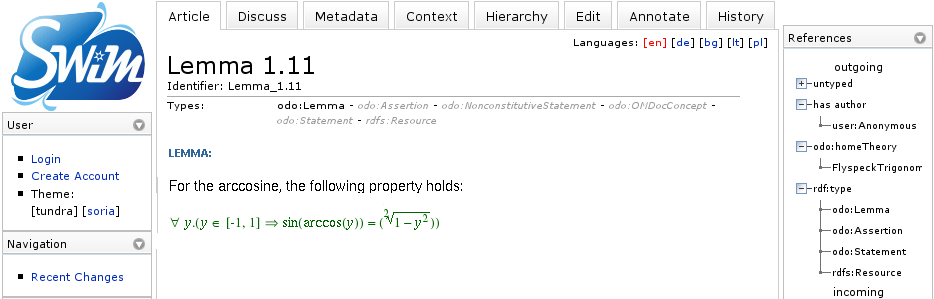
\includegraphics[width=\textwidth]{images/swim-lemma}
  \caption{A Flyspeck lemma in SWiM}
  \label{fig:swim-lemma}
\end{figure}

\paragraph{Prototype} We manually converted part of the trigonometry lemmas to
OMDoc for SWiM (see fig.\ \ref{fig:swim-lemma})\ednote{FYI: Actually only one,
  but we wouldn't have gained more from converting more of them.}  Additionally,
we can auto-generate OMDoc documents from the Twelf source with a converter and
import them into SWiM using the built-in import functionality.

As every SWiM page has an associated discussion page and discussion posts are
semantically represented using the SIOC ontology\cite{SIOC:web}, one can support
the coordination of the project by queries like query~\ref{item:question-count}
from section~\ref{sec:req}.  Work on determining a relevant subset of OMDoc and
its document ontology for discussions is currently in progress\ednote{FYI,
  Florian, this is not a lie but what panta rhei does ;-)}.  Pages and non-OMDoc
links can be annotated with types from ontologies loaded into the
wiki\footnote{Types of OMDoc links are automatically extracted from the markup;
  see above.}.

Authors can embed inline SPARQL queries into wiki pages.  Not all desirable
queries are easy to express in SPARQL; consider query~\ref{item:proven-lemma}:

\begin{lstlisting}
SELECT ?l WHERE { ?l rdf:type odo:Lemma .
                  ?l swrc:isAbout <Composite_Regions> .
                  OPTIONAL { ?p rdf:type odo:Proof .
                             ?p odo:proves ?l . }
                  FILTER ( ! bound(?p) ) }
\end{lstlisting}

This query assumes a SPARQL semantics with negation as
failure\cite{Polleres:SPARQL-Rules07}.

As OMDoc supports all degrees of formalizing mathematical knowledge,
computerized data can be downloaded in their OMDoc representation using SWiM's
export feature and then be converted to Twelf by client-side
software\cite[chap.\ 25.2]{Kohlhase:omdoc1.2}.

\paragraph{Evaluation} Annotating mathematical structures with SWiM is easy---it
just means using the editor and having the annotations extracted.  Other
annotations required for Flyspeck, such as categorizations or progress
information, can be made, but not in an ad-hoc way, which we would have found
useful in the prototyping phase.  Instead, one would have to import an existing
ontology into the wiki, or create it using the build-in ontology editor, and
then one would be able to annotate documents using terms from that ontology.

Browsing is well supported, with incoming and outgoing links being offered for
navigation, and a graphical view of the neighborhood of the current resource in
the RDF graph.

Queries are powerful but not always short and intuitive (see above), but
alternatively, one could just enhance the ontology, harness the power of the
integrated \product{Pellet} OWL-DL reasoner
(see~\cite{KrSchVr:semwiki-reasoning07}), and get the same result with a simple
query for instances of a specially defined class.  For unproven lemmas, the
following axiom would do the trick:

\[
\mbox{LemmaWithoutProof}\equiv\mbox{Lemma}\sqcap\neg(\exists\mbox{proves}^{-1}.\mbox{Proof})
\]

Dependencies can partly be inferred by a DL reasoner, but for a complete support
of OMDoc's notion of dependency, an OMDoc-specific calculus will have to be
applied, which is currently in development.

%%% Local Variables: 
%%% mode: latex
%%% TeX-master: "flyspeck-wiki-eswc08"
%%% End: 


% ---------------------  Related Work  --------------------

\section{Related Work (all)}
\label{sec:related}


\subsection{Management of Mathematical Knowledge}
\label{sec:mkm}

Projects that manage mathematical knowledge can be classified into three groups. The first group comprises projects that do not systematically employ computer support for their management needs. An example for such a projects is the classification of the finite simple groups~\cite{Gorenstein-Lyons-Salomon:1994}. This group could be dubbed the informal group because the produced knowledge, while formal to a large degree, does not exist in a machine-readable form.

The second group is the fully formal group. Projects in this group use computer systems to manipulate the mathematical knowledge. The most important examples for such systems are automated and interactive reasoning tools that permit to construct and search for mathematical proofs. Several such systems are in use, such as Mizar~\cite{mizarmanual}, Coq~\cite{Coq}, or Isabelle~\cite{Isabelle:definition}. For these tools, large libraries, usually with a central repository and a repository viewer, have been developed. For example, the standard Isabelle library covers elementary number theory, analysis, algebra, and set theory. An example or such a project is the fully formal proof of the four color theorem~\cite{Gonthier:FourColor}.

The third group is the semi-formal group. Semi-formal projects try to combine the advantages of the other two groups by formalizing only parts of or only certain aspects of the mathematical. For example, OMDoc and SWiM permit to combine formal mathematical content with natural language in a way that keeps the structure and interfaces of the knowledge machine-readable. This is particularly suited for projects where an informal document is incrementally transformed into a formal one, such as in Flyspeck.

\subsection{Wikis for Mathematics (Christoph)}
\label{sec:math-wiki}

\subsubsection{Semantic Wikis}
\label{sec:semwiki}

Semantic wikis~\cite{semwiki06} are wikis enhanced by semantic annotations.  Although many
ways of semantically enhancing wikis have been investigated, a modeling approach prevails
where one resource (in the RDF sense) --- e.\,g.\ one mathematical theorem --- is
represented by one wiki page and relations between resources by links between pages.  Both
pages and links can be typed with terms from
ontologies~\cite{OrDeMoVoHa06:annotation-navigation-semwiki}, which are either preloaded
into the wiki or modelled ad-hoc~\cite{KrSchVr:semwiki-reasoning07}.  Semantic wikis
commonly offer enhanced navigation capabilities by displaying a summary of all typed
links, grouped by type, with each page.  Most of them allow to search for pages by type or
by them being subject or object of any RDF triple (= typed link), while it depends on the
reasoner used by the wiki whether only explicit RDF triples or also inferred ones are
considered~\cite{KrSchVr:semwiki-reasoning07}.  Such queries can usually be executed
interactively via a special search form, or in an automated way as \emph{inline} queries
embedded into the content of a page.

\subsubsection{Informal Knowledge Collections}
\label{sec:math-knowledge-collections}

Current collaborative projects for managing \emph{informal} mathematical knowledge range
from comprehensive encyclopediæ like the mathematical sections of \product{Wikipedia}\ednote{reference} or
the courseware repository and content management system \product{Connexions}\ednote{reference} to projects
specially focused on mathematics like \product{PlanetMath}\ednote{reference}\footnote{See
  \url{http://www.wikipedia.org}, \url{http://cnx.org} or \url{http://www.planetmath.org},
  respectively.}, which is powered by a highly customized wiki-like system.  The pages in
these systems are categorized and searchable in full-text, with additional metadata
records in the case of \product{PlanetMath}.  Neither of these systems is a
\emph{semantic} wiki, and thus they fail to solve the following two problems, which are
essential for MKM:

\begin{enumerate}
\item\label{item:formula-search-usecase} In \product{Wikipedia} and \product{PlanetMath},
  formulæ are given in presentation-oriented {\LaTeX}.  Imagine a wiki page about the
  Pythagorean Theorem, stated as $a^2 + b^2 = c^2$, and a user searching for the
  equivalent formula $x^2 + y^2 = z^2$ (or even $c=\sqrt{a^2+b^2}$!) --- The system would
  not find the theorem.
\item Neither could ``all theorems about triangles for which a
  proof exists'' be searched for, as the link from a proof to the theorem it proves is not
  typed.
\end{enumerate}

\product{Connexions}, on the other hand, could in principle cope with these two problems,
but in practice it does not: Formulæ are written in the content-oriented sublanguage of
{\mathml}~\cite{CarlisleEd:MathML07}, and the CNXML markup language used for larger
structures allows for annotating texts as mathematical statements like lemmas, but this
structural information is not yet \emph{used} by the system.  Moreover, none of the
systems mentioned so far supports an easy navigation from the occurrence of a mathematical
symbol in a formula to the declaration or definition of this symbol, if it is defined in
some other place of the wiki; instead, the author has to provide links he considers
relevant in the text surrounding the formula.

\subsubsection{Domain-Specific Semantics}
\label{sec:domain-semantics}

Note that general-purpose semantic wikis do not support the above-mentioned use case
(\ref{item:formula-search-usecase}) either, as they neither have a sufficient notion of
equality nor understand mathematical content markup.  If we assume ``semantic'' not just
to mean RDF or description logics, but any kind of (higher-order) logic required for
specific domains\ednote{@Florian: This is quite superficial, can we write it in a more
  sophisticated way?} and employ domain-specific ways of knowledge representation we can
imagine semantic wikis specifically supporting mathematics.  For use case
(\ref{item:formula-search-usecase}), we could have the wiki pages crawled by a formula
search engine like MathWebSearch~\cite{KohSuc:asemf06}, which applies substitution tree
indexing to mathematical formulae.  Even more formal approaches integrate automated
theorem provers into wikis.  Two of these systems are discussed in
section~\ref{sec:wiki-pa}.


\subsection{Wikis with Integrated Proof Assistants}
\label{sec:wiki-pa}

Recently, there is a growing interest in integrating automated theorem provers or proof
assistants with wikis\footnote{See \url{http://homepages.inf.ed.ac.uk/da/mathwiki/} for
  relevant activities.}.  Both Logiweb and ProofWiki are wiki-like systems that support
checking or interactive development of proofs.  Both are ``semantic'' in the sense that
the integrated proof checker can utilize the mathematical knowledge in the wiki pages.
But the semantics is not utilized for purposes other than that, such as facilitating
browsing or editing, or connecting to services on the semantic web.  Developing and
verifying formal proofs in the wiki is not yet the focus of Flyspeck in this early stage,
but it may be required later if the central maintainer approach does not turn out to work.

\paragraph{Logiweb} is a distributed system for publishing machine checked mathematics in
high-quality PDF~\cite{Grue:Logiweb07}.  While the author does not call it a ``wiki'', it
shares part of the key wiki principles: Anybody can contribute to a Logiweb site and edit
new pages in a simple text syntax with a browser.  On the other hand, Logiweb does not
offer other features that would be essential for Flyspeck: browsing by traversing links is
supported neither in the editor nor in the generated PDF, and Logiweb does not offer a
built-in search or query facility.  Logiweb does not allow for \emph{exchanging} knowledge
as required for Flyspeck: Documents can be exported in presentational formats like PDF or
\TeX{}, and their internal, low-level data structures can be exported as XML or Lisp
S-expressions, but currently there is no easy way to convert these representations to
other languages for mathematical markup or theorem proving.  Finally, the way Logiweb
checks proofs is not compatible with other theorem provers, as all calculi and proof
tactics need to be defined in the Logiweb system itself.

\paragraph{ProofWiki} is an integration of ProofWeb, a web frontend to the Coq proof
assistant, into MediaWiki~\cite{CorKal:CoopReposFormalProofs07}.  Coq's converting tools
are used to generate human-readable and browsable HTML or {\LaTeX} presentation from the proof
scripts.  In the HTML generated that way, symbols are linked to their declaration.  Index
pages, such as lists of all definitions or all theorems, are generated, but their
generation cannot be influenced or customized through the wiki
interface\ednote{@Christoph: check!}.  So far, there is just text search, and dependencies
among knowledge items are only computed for exporting proof scripts but not used for
browsing inside the system.  Another disadvantage of ProofWiki in the context of Flyspeck
is that pages can either be formal proof scripts (with restricted possibilities to include
informal comments), or informal wiki pages.  Semi-formal documents or stepwise formalizing
of knowledge is not supported.  Importing and exporting Coq proof scripts to and from the
wiki is possible, but other formats are not yet supported.  While the authors do provide
instructions on how to integrate other theorem provers, doing so would be a lot of work,
as there is no abstraction layer or metalanguage for exchanging or converting data.

\ednote{@Christoph: Find out whether such systems have already been used in Flyspeck-like
  scenarios, i.\,e.\ collaboratively proving something.}

%%% Local Variables: 
%%% mode: latex
%%% fill-column: 90
%%% TeX-master: "flyspeck-wiki-eswc08"
%%% End: 


% ---------------------  Conclusion  ----------------------


\section{Conclusion and Further Work}
\label{sec:conc}

Our preliminary experiments lead us to believe that, due to its rich
semantic web and OMDoc infrastructure, future work toward supporting
Flyspeck should continue in the SWiM infrastructure.  For the text-based
page format of MediaWiki, features that rely on structures like the
linking of symbols could only be realized in an ad hoc way
using, say, regular expressions.  Relying on the XML infrastructure of
OMDoc, these features are either already available or easier to develop.
However, rapidly \emph{prototyping} our first ideas about the wiki
support required for Flyspeck was easier in Semantic MediaWiki due to
its ability to design ad hoc ontologies and its implementation in the
interpreted language PHP.

\paragraph{Importing} For this case study, we created OMDoc from Twelf. OMDoc
also offers support for the alternative workflow of stepwise formalization as
well.  One could either start by converting the Flyspeck book from {\LaTeX} to
HTML with Presentation MathML formulæ and formalize the presentation markup into
content markup step by step, or one could start the formalization on the {\TeX}
side.  There, one would formalize the book to s\TeX{}, a content-oriented {\TeX}
notation for OMDoc, which can then be converted to OMDoc\cite{Kohlhase:albwo06}.
Either way involves a {\TeX}-to-XML transformation, which has been tested in
large scale in our group\cite{URL:arXMLiv}.

\paragraph{Annotating} 

Using the module system of OMDoc could help to simplify
the structure of the proof. In any case it can be used to explicate
the dependencies between components of the proof. 

\ednote{@Christoph: Needs to support both preloaded and ad-hoc
  ontologies: The OMDoc document ontology is preloaded, while other
  annotations can be added at will. (Make SWiM more ``wiki''!)}

More ontology-powered services, particularly ones that facilitate editing
documents, are planned for version 0.3\cite{swim-roadmap,Lange:SWiMSciColl07}

\paragraph{Browsing}

\ednote{@Christoph: narrative structure: do not use ad hoc categories, but OMDoc's native
  NarCons\cite{KohMueMue:dfncimk07}; need to be added to document ontology.}

\paragraph{Querying} Additionally, proof search will be greatly simplified if
the semantic-aware search engine MathWebSearch\cite{KohSuc:asemf06} is used,
which applies substitution tree indexing to mathematical formulae.  That means,
for example, that a query for $\int f(x) dx$ would also find $\int f(y) dy$.

\paragraph{Download} If several parts of the proof are done in different
theorem provers, highly non-trivial and mostly novel translations become
necessary to provide one single proof object. Here OMDoc could be used as an
exchange format between theorem prover languages, and formal translations could
be specified in OMDoc itself.  While this line of research is interesting, it is
difficult for us to forsee what kinds of translations, if any, will be needed.

Dependencies can partly be inferred by a DL reasoner, but for a complete support
of OMDoc's notion of dependency, an OMDoc-specific calculus will have to be
applied, which is currently in development.

\paragraph{Upload} Needs investigation; see related work.

%%% Local Variables: 
%%% mode: latex
%%% TeX-master: "flyspeck-wiki-eswc08"
%%% End: 


\paragraph{Acknowledgments}
\label{sec:ack}

\begin{itemize}
\item Michael Kohlhase
\item Immanuel Normann
\item Stefan Decker
\end{itemize}

\bibliographystyle{abbrv}
% load crossrefs last when using modular bib files
\bibliography{flyspeck-wiki,seanbib/all}

% \printindex

\ednotemessage
\end{document}

% vim:tw=90:autoindent: 
%%% Local Variables: 
%%% mode: latex
%%% End: 
